\documentclass{article}
\usepackage{url,color,xspace,verbatim,subfig,ctable,multirow,listings}
\usepackage[utf8]{inputenc}
\usepackage[T1]{fontenc}
\usepackage{txfonts}
\usepackage{rotating}
\usepackage{paralist}
\usepackage{subfig}
\usepackage{graphics}
\usepackage{enumitem}
\usepackage{times}
\usepackage{amssymb}
\usepackage[colorlinks=true]{hyperref}
\usepackage[ruled,vlined]{algorithm2e}

% ==================================================

\graphicspath{{figs/}}
\urlstyle{sf}

% tikz stuff
\usepackage{tikz}
\usepackage{pgfplots}
% configuration
\usetikzlibrary{shapes,positioning,calc,snakes,arrows,shapes}
\pgfplotsset{width=.9\linewidth}

\lstset{
  language=C,
  basicstyle=\ttfamily \small,
  flexiblecolumns=false,
  basewidth={0.5em,0.45em},
  boxpos=t,
}

\newcommand{\etal}{{\it et al.}\xspace}
\newcommand{\naive}{na\"{\i}ve\xspace}
\newcommand{\Naive}{Na\"{\i}ve\xspace}
\newcommand{\textc}[1]{{\color{gray} {\footnotesize #1}}}

\definecolor{skRed}{RGB}{155,25,25}
\newcommand{\stefan}[1]{
  {\color{skRed}[{\color{red}{SK}} #1]}}

\setcounter{section}{0} % Start sections with 1, not 0
\begin{document}

\title{Adaptive broadcast tree for multicores}

% email address
\newcommand{\eaddr}{stefan.kaestle@inf.ethz.ch}
\newcommand{\email}{\href{mailto:\eaddr}{\eaddr}}

\author{Stefan Kaestle\\
  \email \\
  Systems Group, ETH Zurich}

\maketitle

%%%%%%%%%%%%%%%%%%%%%%%%%%%%%%%%%%%%%%%%%%%%%%%%%%
%%%%%%%%%%%%%%%%%%%%%%%%%%%%%%%%%%%%%%%%%%%%%%%%%%
\section{Introduction}

Atomic broadcast is a building-block for many higher-level distributed
algorithm such as state-machine replication. Such distributed
algorithms are increasingly used to overcome scalability challenges on
multicore machines. Examples are databases~\cite{Salomie2011,
  Wiesmann2000} and operating systems~\cite{fos:osr09, tornado:osdi99,
  barrelfish:sosp09}.

% What do you want to enable?
We want to investigate how to achieve better performance of atomic
broadcast across a wide range of multicore machines without manually
tuning the implementation to concrete machines.

% What problem are you solving, and why is it hard?
The problem is complexity and diversity of modern multicore
machines. Multicores come in many flavors depending on vendor and
generation of the machine. All of these machines have fundamentally
different characteristics such as number of nodes, NUMA
characteristics, interconnect topologies, propagation time on
interconnect and use of shared caches. These characteristics are hard
to understand, but important to consider for application performance. 

% New ideas
Instead of manually tuning algorithms to characteristics of individual
machines, we automatically configure our atomic broadcast
implementation based on a machine model.
% How will you go about it?
We will base our atomic broadcast on overlay networks, which we
automatically configure based on the machine model. One questions is
which information should actually be encoded in the machine model. %
Our idea is to then explore different approaches (such as MST
algorithms, clustering) to \emph{find good overlay networks} based on
the network model to base the atomic broadcast on. Then, for every
node, we need to decide which message to send first. This is a
\emph{scheduling} problem.

% How do we show it works
We auto-configure a wide range of different multicore machines and
show the performance of our implementation comes close to the
performance of hand-tuned implementations for all of these machines.

% Hypothesis
My hypothesis is that automatic tuning of atomic broadcast (and other
distributed algorithms) to machine characteristics is worth
doing. Obviously, we cannot achieve performance of hand-tuned
implementations, but we can get close enough to argue that loosing a
bit of performance to avoid tedious manual reconfiguration is worth if
for many applications (while others, where performance \emph{really}
matters, might still want to manually configure their stuff).

%%%%%%%%%%%%%%%%%%%%%%%%%%%%%%%%%%%%%%%%%%%%%%%%%%
%%%%%%%%%%%%%%%%%%%%%%%%%%%%%%%%%%%%%%%%%%%%%%%%%%
\section{Related work}

A multicore aware broadcast has been implemented in~\cite{Tu2008}. It
takes the cache architecture of the machine (and only one particular?)
into consideration for building the broadcast. It is however for
larger messages (starting at 4K) and it does not seem to be performing
very well (numbers are given in microseconds -6). 4K messages are 52
microseconds, which is 150000 cycles. For synchronization primitives,
a cache line is sufficient.

Another tree implementation with MPI in mind was done
in~\cite{Graham2008}. They have comparable numbers to what we found,
but they cannot automatically tune to different machine
characteristics. Our hypothesis is that we can do achieve higher
average performance across a wide range of different multicore
machines without manually adapting the implementation.

Alistarh\etal~\cite{Alistarh2012} show composition of shared-memory
algorithms that perform efficiently under different conditions at
negligible overhead. A similar approach can potentially be applied to
deal with diversity of multicore machines. However, we would have
to extend it to support both shared-memory and message-passing
implementations. 

%%%%%%%%%%%%%%%%%%%%%%%%%%%%%%%%%%%%%%%%%%%%%%%%%%
%%%%%%%%%%%%%%%%%%%%%%%%%%%%%%%%%%%%%%%%%%%%%%%%%%
\section{The multicore network model}

% selecting hard
Characteristics of the network influence the performance of
distributed algorithms. Due to the heterogeneous combinations of
complex networks on multicores, selection of algorithms is
particularly hard.

% model
We express the network characteristics in a multicore network
model. This model at this stage is by no means complete. We are going to
extend it over time to address more complexities of current and future
multicores.

% graph
We represent the multicore network as a graph. The nodes in this graph
correspond to cores, and edges the communication channels between
nodes. The machines we consider for now only have bi-directional
communication links. Other machines (like the SCC) have
uni-directional links, which is why we model the graph as directed
graph.

% shared memory -> fully meshed
This graph is fully meshed for shared memory machines. Every core can
communicate with every other node via the cache coherence protocol.

%%%%%%%%%%%%%%%%%%%%%%%%%%%%%%%%%%%%%%%%%%%%%%%%%%
\subsection{Node characteristics} 
\label{sec:model_nodes}

Every node (i.e.\ core) in the system has characteristics associated
with it:

\begin{description}
\item[synchrony] Parts of a multicore machine are synchronous. Hence,
  one characteristic of a node is an identifier for the synchrony
  cluster of a node.
\item[send time $t_{send}$] Time required to send a message, i.e.\ marshalling
  and queuing the message
\item[receive $t_{recv}$] Time required to receive a message, i.e.\
  dequeuing, unmarshalling and demultiplexing a channel.
\item[failure] Can nodes fail? If so, how? (Byzantine, crash)
\end{description}

%%%%%%%%%%%%%%%%%%%%%%%%%%%%%%%%%%%%%%%%%%%%%%%%%%
\subsection{Link characteristics} 
\label{sec:model_links}

The network model is defined by communication channels, which in turn
are defined by a set of attributes (here sorted by priority):

\begin{description}
\item[latency] (quantitative) between each pair of nodes (per-edge)
\item[breakdown] (quantitative) of message send cost:
  dominating propagation time vs.\ dominating send and receive time on
  multicores (per-node)
\item[bounded delivery]
\item[reliability] (loss, link failure, in-order delivery, phantoms,
  corruption, duplicated messages): 
  multicore interconnect networks often are
\end{description}

% Assumptions
We assume that the cost of sending a message to the same node is 0,
which is not true, since even using a highly optimized implementation
for local communication (like LMP) has a non-negligible cost.

% Limitations
What we do not consider yet is link congestion. 

%%%%%%%%%%%%%%%%%%%%%%%%%%%%%%%%%%%%%%%%%%%%%%%%%%
\subsection{Hierarchical model}
\label{sec:model_hierarchy}

Multicore machines are hierarchical. Processor cores are grouped in
NUMA nodes with shared caches. These NUMA nodes are then connected to
each other by increasingly complex interconnect networks. 

We encode NUMA node affinity in our model. This allows to break down
programming of a multicore machine into two distinct instances. We
solve one instance of the problem between NUMA nodes, and then, in a
second step, within each NUMA node. These two steps can be executed
independently and different algorithms can be used in both case.

If cores on the same NUMA node share a cache, it makes sense to
leverage this hardware feature to implement shared-memory algorithms
on top of it. %
Communication across NUMA nodes is realized sending messages across
the packet-based interconnect network. Using message-passing based
implementations is the natural choice. %
Shared memory algorithms and message-passing based algorithms can be
composed together to program hierarchical machines similarly to what
was previously shown for composing of shared-memory
algorithms~\cite{Alistarh2012}.

%%%%%%%%%%%%%%%%%%%%%%%%%%%%%%%%%%%%%%%%%%%%%%%%%%
\subsection{Acquiring the model}

% Model given
We assume that the model is given. We just define one ourselves for
now or build one manually for a particular machine. In a real-world
scenario, this does not work. The model needs to be created
automatically for a particular machine (due to the diversity of
machines, and also the pace at which hardware changes)

We now make up a machine model for evaluation. This model is based on
a 8x4x1 AMD Shanghai machine. The topology of such a machine is shown
in Figure~\ref{fig:gruyere}.

Each of the eight nodes consists of four cores. We approximate the
cost of sending messages within nodes as $1$ and across nodes as
$10*num(hops)$.

Send and receive time are $10$ each, i.e.\ in the order of propagation
over a cross-NUMA link.

\begin{figure}[htb]
  \centering
  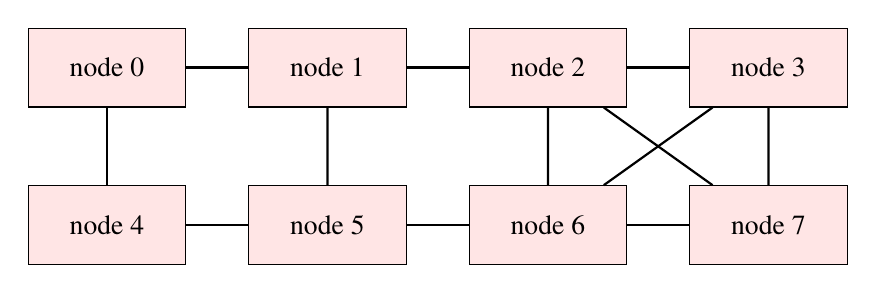
\begin{tikzpicture}[
    xscale=.7,
    yscale=.5,
    every node/.style={draw,fill=red!10,minimum width=2cm,minimum height=1cm}
    ]
    \node (c1) at ( 0, 4) {node 0};
    \node (c2) at ( 4, 4) {node 1};
    \node (c3) at ( 8, 4) {node 2};
    \node (c4) at (12, 4) {node 3};

    \node (c5) at ( 0, 0) {node 4};
    \node (c6) at ( 4, 0) {node 5};
    \node (c7) at ( 8, 0) {node 6};
    \node (c8) at (12, 0) {node 7};

    % top horizontal
    \draw[thick] (c1) -- (c2);
    \draw[thick] (c2) -- (c3);
    \draw[thick] (c3) -- (c4);
    % bottom horizontal
    \draw[thick] (c5) -- (c6);
    \draw[thick] (c6) -- (c7);
    \draw[thick] (c7) -- (c8);
    % vertical
    \draw[thick] (c1) -- (c5);
    \draw[thick] (c2) -- (c6);
    \draw[thick] (c3) -- (c7);
    \draw[thick] (c4) -- (c8);
    % cross
    \draw[thick] (c3) -- (c8);
    \draw[thick] (c4) -- (c7);
  \end{tikzpicture}
  \caption{Interconnect topology of 8x4x1 AMD Shanghai machine}
  \label{fig:gruyere}
\end{figure}

%%%%%%%%%%%%%%%%%%%%%%%%%%%%%%%%%%%%%%%%%%%%%%%%%%
%%%%%%%%%%%%%%%%%%%%%%%%%%%%%%%%%%%%%%%%%%%%%%%%%%
\section{Atomic Broadcast for Multicores}

For a specific model, we now need to find ``the right'' implementation
of algorithms to program it. We build our atomic broadcast based on a
subset of links offered by the model such that all nodes of a given
multicore machine can be reached. Atomic broadcast guarantees that 1)
if one node receives a message, all other nodes receive it as well,
and 2) that all nodes see the message in the same order.

First, we discuss what kind of topologies we use to communicate
between nodes. We evaluate tree based implementations. Other
potentially interesting topologies are rings.

%%%%%%%%%%%%%%%%%%%%%%%%%%%%%%%%%%%%%%%%%%%%%%%%%%
\subsection{Tree Topology}

We now look at tree-based atomic broadcast implementations. The first
challenge is to find efficient spanning trees for arbitrary
machines. We now discuss different strategies to select trees based on
the model representing the machine.

%-------------------------------------------------
\subsubsection{Binary Tree}

A very \naive strategy to build a tree from machine models is the use
of a binary tree with root in core 0. Every node $n$ has two children
$2(n+1)-1$ and $2(n+1)$.

The benefit of such a tree is that the time complexity is guaranteed
to be $O(\log{n})$. The downside is that it is not considering the
machine topology. Unnecessary communication across NUMA nodes might be
introduced. 

We show an example for such a tree for a 8x4x1 AMD Barcelona machine
(gruyere) in Figure~\ref{fig:qrm_tree_gruyere}.

\begin{figure}
  % Start of code
% \begin{tikzpicture}[anchor=mid,>=latex',line join=bevel,]
\begin{tikzpicture}[>=latex',line join=bevel,scale=.35]
  \pgfsetlinewidth{1bp}
%%
\pgfsetcolor{black}
  % Edge: 15 -> 31
  \draw [->] (27bp,74.327bp) .. controls (27bp,66.264bp) and (27bp,56.648bp)  .. (27bp,37.667bp);
  % Edge: 9 -> 19
  \draw [->] (459bp,148.33bp) .. controls (459bp,140.26bp) and (459bp,130.65bp)  .. (459bp,111.67bp);
  % Edge: 14 -> 30
  \draw [->] (1050.3bp,151.31bp) .. controls (1060.4bp,140.94bp) and (1073.7bp,127.18bp)  .. (1092bp,108.42bp);
  % Edge: 14 -> 29
  \draw [->] (1035bp,148.33bp) .. controls (1035bp,140.26bp) and (1035bp,130.65bp)  .. (1035bp,111.67bp);
  % Edge: 11 -> 23
  \draw [->] (659.73bp,151.31bp) .. controls (649.64bp,140.94bp) and (636.25bp,127.18bp)  .. (618bp,108.42bp);
  % Edge: 7 -> 15
  \draw [->] (83.731bp,151.31bp) .. controls (73.64bp,140.94bp) and (60.253bp,127.18bp)  .. (42bp,108.42bp);
  % Edge: 0 -> 2
  \draw [->] (588.87bp,377.76bp) .. controls (613.22bp,365.25bp) and (652.76bp,344.93bp)  .. (689.4bp,326.1bp);
  % Edge: 10 -> 22
  \draw [->] (387bp,148.33bp) .. controls (387bp,140.26bp) and (387bp,130.65bp)  .. (387bp,111.67bp);
  % Edge: 13 -> 28
  \draw [->] (935.71bp,149.09bp) .. controls (939.96bp,140.36bp) and (945.15bp,129.68bp)  .. (954.37bp,110.75bp);
  % Edge: 1 -> 3
  \draw [->] (398.64bp,306.66bp) .. controls (360.05bp,293.43bp) and (284.76bp,267.64bp)  .. (231.27bp,249.31bp);
  % Edge: 6 -> 14
  \draw [->] (946.31bp,227.77bp) .. controls (963.36bp,216.09bp) and (988.4bp,198.93bp)  .. (1015.9bp,180.12bp);
  % Edge: 3 -> 8
  \draw [->] (207bp,222.33bp) .. controls (207bp,214.26bp) and (207bp,204.65bp)  .. (207bp,185.67bp);
  % Edge: 13 -> 27
  \draw [->] (918.29bp,149.09bp) .. controls (914.04bp,140.36bp) and (908.85bp,129.68bp)  .. (899.63bp,110.75bp);
  % Edge: 10 -> 21
  \draw [->] (371.73bp,151.31bp) .. controls (361.64bp,140.94bp) and (348.25bp,127.18bp)  .. (330bp,108.42bp);
  % Edge: 12 -> 26
  \draw [->] (762.27bp,151.31bp) .. controls (772.36bp,140.94bp) and (785.75bp,127.18bp)  .. (804bp,108.42bp);
  % Edge: 3 -> 7
  \draw [->] (187.69bp,227.77bp) .. controls (170.64bp,216.09bp) and (145.6bp,198.93bp)  .. (118.14bp,180.12bp);
  % Edge: 5 -> 12
  \draw [->] (719.71bp,223.09bp) .. controls (723.96bp,214.36bp) and (729.15bp,203.68bp)  .. (738.37bp,184.75bp);
  % Edge: 9 -> 20
  \draw [->] (474.27bp,151.31bp) .. controls (484.36bp,140.94bp) and (497.75bp,127.18bp)  .. (516bp,108.42bp);
  % Edge: 1 -> 4
  \draw [->] (423bp,296.33bp) .. controls (423bp,288.26bp) and (423bp,278.65bp)  .. (423bp,259.67bp);
  % Edge: 0 -> 1
  \draw [->] (545.13bp,377.76bp) .. controls (520.78bp,365.25bp) and (481.24bp,344.93bp)  .. (444.6bp,326.1bp);
  % Edge: 2 -> 5
  \draw [->] (711bp,296.33bp) .. controls (711bp,288.26bp) and (711bp,278.65bp)  .. (711bp,259.67bp);
  % Edge: 11 -> 24
  \draw [->] (675bp,148.33bp) .. controls (675bp,140.26bp) and (675bp,130.65bp)  .. (675bp,111.67bp);
  % Edge: 4 -> 10
  \draw [->] (414.29bp,223.09bp) .. controls (410.04bp,214.36bp) and (404.85bp,203.68bp)  .. (395.63bp,184.75bp);
  % Edge: 12 -> 25
  \draw [->] (747bp,148.33bp) .. controls (747bp,140.26bp) and (747bp,130.65bp)  .. (747bp,111.67bp);
  % Edge: 8 -> 17
  \draw [->] (198.29bp,149.09bp) .. controls (194.04bp,140.36bp) and (188.85bp,129.68bp)  .. (179.63bp,110.75bp);
  % Edge: 6 -> 13
  \draw [->] (927bp,222.33bp) .. controls (927bp,214.26bp) and (927bp,204.65bp)  .. (927bp,185.67bp);
  % Edge: 5 -> 11
  \draw [->] (702.29bp,223.09bp) .. controls (698.04bp,214.36bp) and (692.85bp,203.68bp)  .. (683.63bp,184.75bp);
  % Edge: 7 -> 16
  \draw [->] (99bp,148.33bp) .. controls (99bp,140.26bp) and (99bp,130.65bp)  .. (99bp,111.67bp);
  % Edge: 2 -> 6
  \draw [->] (735.36bp,306.66bp) .. controls (773.95bp,293.43bp) and (849.24bp,267.64bp)  .. (902.73bp,249.31bp);
  % Edge: 8 -> 18
  \draw [->] (215.71bp,149.09bp) .. controls (219.96bp,140.36bp) and (225.15bp,129.68bp)  .. (234.37bp,110.75bp);
  % Edge: 4 -> 9
  \draw [->] (431.71bp,223.09bp) .. controls (435.96bp,214.36bp) and (441.15bp,203.68bp)  .. (450.37bp,184.75bp);
  % Node: 24
\begin{scope}
  \definecolor{strokecol}{rgb}{0.0,0.0,0.0};
  \pgfsetstrokecolor{strokecol}
  \draw (675bp,93bp) ellipse (27bp and 18bp);
  \draw (675bp,93bp) node {24};
\end{scope}
  % Node: 25
\begin{scope}
  \definecolor{strokecol}{rgb}{0.0,0.0,0.0};
  \pgfsetstrokecolor{strokecol}
  \draw (747bp,93bp) ellipse (27bp and 18bp);
  \draw (747bp,93bp) node {25};
\end{scope}
  % Node: 26
\begin{scope}
  \definecolor{strokecol}{rgb}{0.0,0.0,0.0};
  \pgfsetstrokecolor{strokecol}
  \draw (819bp,93bp) ellipse (27bp and 18bp);
  \draw (819bp,93bp) node {26};
\end{scope}
  % Node: 27
\begin{scope}
  \definecolor{strokecol}{rgb}{0.0,0.0,0.0};
  \pgfsetstrokecolor{strokecol}
  \draw (891bp,93bp) ellipse (27bp and 18bp);
  \draw (891bp,93bp) node {27};
\end{scope}
  % Node: 20
\begin{scope}
  \definecolor{strokecol}{rgb}{0.0,0.0,0.0};
  \pgfsetstrokecolor{strokecol}
  \draw (531bp,93bp) ellipse (27bp and 18bp);
  \draw (531bp,93bp) node {20};
\end{scope}
  % Node: 21
\begin{scope}
  \definecolor{strokecol}{rgb}{0.0,0.0,0.0};
  \pgfsetstrokecolor{strokecol}
  \draw (315bp,93bp) ellipse (27bp and 18bp);
  \draw (315bp,93bp) node {21};
\end{scope}
  % Node: 22
\begin{scope}
  \definecolor{strokecol}{rgb}{0.0,0.0,0.0};
  \pgfsetstrokecolor{strokecol}
  \draw (387bp,93bp) ellipse (27bp and 18bp);
  \draw (387bp,93bp) node {22};
\end{scope}
  % Node: 23
\begin{scope}
  \definecolor{strokecol}{rgb}{0.0,0.0,0.0};
  \pgfsetstrokecolor{strokecol}
  \draw (603bp,93bp) ellipse (27bp and 18bp);
  \draw (603bp,93bp) node {23};
\end{scope}
  % Node: 28
\begin{scope}
  \definecolor{strokecol}{rgb}{0.0,0.0,0.0};
  \pgfsetstrokecolor{strokecol}
  \draw (963bp,93bp) ellipse (27bp and 18bp);
  \draw (963bp,93bp) node {28};
\end{scope}
  % Node: 29
\begin{scope}
  \definecolor{strokecol}{rgb}{0.0,0.0,0.0};
  \pgfsetstrokecolor{strokecol}
  \draw (1035bp,93bp) ellipse (27bp and 18bp);
  \draw (1035bp,93bp) node {29};
\end{scope}
  % Node: 1
\begin{scope}
  \definecolor{strokecol}{rgb}{0.0,0.0,0.0};
  \pgfsetstrokecolor{strokecol}
  \draw (423bp,315bp) ellipse (27bp and 18bp);
  \draw (423bp,315bp) node {1};
\end{scope}
  % Node: 0
\begin{scope}
  \definecolor{strokecol}{rgb}{0.0,0.0,0.0};
  \pgfsetstrokecolor{strokecol}
  \draw (567bp,389bp) ellipse (27bp and 18bp);
  \draw (567bp,389bp) node {0};
\end{scope}
  % Node: 3
\begin{scope}
  \definecolor{strokecol}{rgb}{0.0,0.0,0.0};
  \pgfsetstrokecolor{strokecol}
  \draw (207bp,241bp) ellipse (27bp and 18bp);
  \draw (207bp,241bp) node {3};
\end{scope}
  % Node: 2
\begin{scope}
  \definecolor{strokecol}{rgb}{0.0,0.0,0.0};
  \pgfsetstrokecolor{strokecol}
  \draw (711bp,315bp) ellipse (27bp and 18bp);
  \draw (711bp,315bp) node {2};
\end{scope}
  % Node: 5
\begin{scope}
  \definecolor{strokecol}{rgb}{0.0,0.0,0.0};
  \pgfsetstrokecolor{strokecol}
  \draw (711bp,241bp) ellipse (27bp and 18bp);
  \draw (711bp,241bp) node {5};
\end{scope}
  % Node: 4
\begin{scope}
  \definecolor{strokecol}{rgb}{0.0,0.0,0.0};
  \pgfsetstrokecolor{strokecol}
  \draw (423bp,241bp) ellipse (27bp and 18bp);
  \draw (423bp,241bp) node {4};
\end{scope}
  % Node: 7
\begin{scope}
  \definecolor{strokecol}{rgb}{0.0,0.0,0.0};
  \pgfsetstrokecolor{strokecol}
  \draw (99bp,167bp) ellipse (27bp and 18bp);
  \draw (99bp,167bp) node {7};
\end{scope}
  % Node: 6
\begin{scope}
  \definecolor{strokecol}{rgb}{0.0,0.0,0.0};
  \pgfsetstrokecolor{strokecol}
  \draw (927bp,241bp) ellipse (27bp and 18bp);
  \draw (927bp,241bp) node {6};
\end{scope}
  % Node: 9
\begin{scope}
  \definecolor{strokecol}{rgb}{0.0,0.0,0.0};
  \pgfsetstrokecolor{strokecol}
  \draw (459bp,167bp) ellipse (27bp and 18bp);
  \draw (459bp,167bp) node {9};
\end{scope}
  % Node: 8
\begin{scope}
  \definecolor{strokecol}{rgb}{0.0,0.0,0.0};
  \pgfsetstrokecolor{strokecol}
  \draw (207bp,167bp) ellipse (27bp and 18bp);
  \draw (207bp,167bp) node {8};
\end{scope}
  % Node: 11
\begin{scope}
  \definecolor{strokecol}{rgb}{0.0,0.0,0.0};
  \pgfsetstrokecolor{strokecol}
  \draw (675bp,167bp) ellipse (27bp and 18bp);
  \draw (675bp,167bp) node {11};
\end{scope}
  % Node: 10
\begin{scope}
  \definecolor{strokecol}{rgb}{0.0,0.0,0.0};
  \pgfsetstrokecolor{strokecol}
  \draw (387bp,167bp) ellipse (27bp and 18bp);
  \draw (387bp,167bp) node {10};
\end{scope}
  % Node: 13
\begin{scope}
  \definecolor{strokecol}{rgb}{0.0,0.0,0.0};
  \pgfsetstrokecolor{strokecol}
  \draw (927bp,167bp) ellipse (27bp and 18bp);
  \draw (927bp,167bp) node {13};
\end{scope}
  % Node: 12
\begin{scope}
  \definecolor{strokecol}{rgb}{0.0,0.0,0.0};
  \pgfsetstrokecolor{strokecol}
  \draw (747bp,167bp) ellipse (27bp and 18bp);
  \draw (747bp,167bp) node {12};
\end{scope}
  % Node: 15
\begin{scope}
  \definecolor{strokecol}{rgb}{0.0,0.0,0.0};
  \pgfsetstrokecolor{strokecol}
  \draw (27bp,93bp) ellipse (27bp and 18bp);
  \draw (27bp,93bp) node {15};
\end{scope}
  % Node: 14
\begin{scope}
  \definecolor{strokecol}{rgb}{0.0,0.0,0.0};
  \pgfsetstrokecolor{strokecol}
  \draw (1035bp,167bp) ellipse (27bp and 18bp);
  \draw (1035bp,167bp) node {14};
\end{scope}
  % Node: 17
\begin{scope}
  \definecolor{strokecol}{rgb}{0.0,0.0,0.0};
  \pgfsetstrokecolor{strokecol}
  \draw (171bp,93bp) ellipse (27bp and 18bp);
  \draw (171bp,93bp) node {17};
\end{scope}
  % Node: 16
\begin{scope}
  \definecolor{strokecol}{rgb}{0.0,0.0,0.0};
  \pgfsetstrokecolor{strokecol}
  \draw (99bp,93bp) ellipse (27bp and 18bp);
  \draw (99bp,93bp) node {16};
\end{scope}
  % Node: 19
\begin{scope}
  \definecolor{strokecol}{rgb}{0.0,0.0,0.0};
  \pgfsetstrokecolor{strokecol}
  \draw (459bp,93bp) ellipse (27bp and 18bp);
  \draw (459bp,93bp) node {19};
\end{scope}
  % Node: 18
\begin{scope}
  \definecolor{strokecol}{rgb}{0.0,0.0,0.0};
  \pgfsetstrokecolor{strokecol}
  \draw (243bp,93bp) ellipse (27bp and 18bp);
  \draw (243bp,93bp) node {18};
\end{scope}
  % Node: 31
\begin{scope}
  \definecolor{strokecol}{rgb}{0.0,0.0,0.0};
  \pgfsetstrokecolor{strokecol}
  \draw (27bp,19bp) ellipse (27bp and 18bp);
  \draw (27bp,19bp) node {31};
\end{scope}
  % Node: 30
\begin{scope}
  \definecolor{strokecol}{rgb}{0.0,0.0,0.0};
  \pgfsetstrokecolor{strokecol}
  \draw (1107bp,93bp) ellipse (27bp and 18bp);
  \draw (1107bp,93bp) node {30};
\end{scope}
%
\end{tikzpicture}
% End of code




  \caption{\Naive binary tree of cores for broadcast on gruyere}
  \label{fig:qrm_tree_gruyere}
\end{figure}

%-------------------------------------------------
\subsubsection{Minimum-Spanning Tree}
\label{sec:mst_tree}

We can apply a minimum spanning tree algorithm to the machine model
graph to find a number of links such that these links connect all
nodes at a minimum cost.

We have implemented such an algorithm and found out, that it is not a
good solution in the general case, since it does not consider
parallelism. Naturally, we would like to parallelize send operations
to different nodes, which allows them to send messages in parallel. 

An example is obvious in Figure~\ref{fig:mst_gruyere_operations}. The
level of parallelism is only two. Cores 00 to 15 are dealt with in
parallel to cores 16 to 31. Other than that, there is no further
parallelism although it is possible to ``split up'' communication with
every new ``round'' (i.e.\ send operations of nodes).

An important variable in constructing such a tree is the degree of
nodes. If the send cost $t_s$ is smaller than the propagation time
$t_p$, $d = \lfloor \frac{t_p}{t_s} \rfloor$ messages can be send to
hide propagation of messages. Hence, a tree with degree $d$ should be
ideal to minimize latency. For multicore interconnect networks,
however, we expect $d<1$. Thus, we do not look into this in detail
right now.

Reducing the degree of nodes also helps for the select operation. It
reduces the number of memory locations to poll, and therefore the
latency of detecting messages.

We show the multicast tree automatically generated from a fully meshed
machine model by applying a minimum spanning tree algorithm in
Figure~\ref{fig:mst_gruyere}.

\begin{figure}
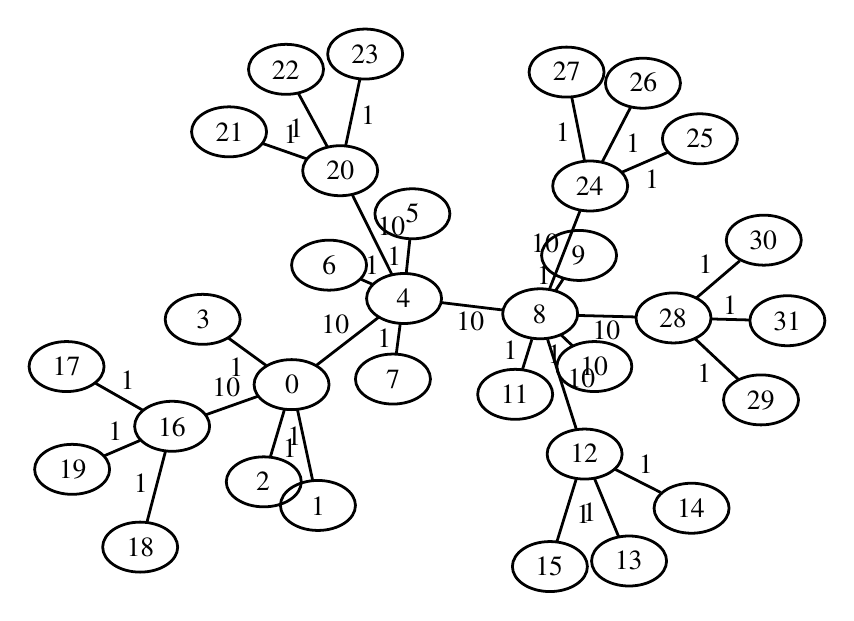
\begin{tikzpicture}[>=latex,line join=bevel,scale=.5]
  \pgfsetlinewidth{1bp}
%%
\pgfsetcolor{black}
  % Edge: 0 -- 16
  \draw [] (166.21bp,141.75bp) .. controls (154.21bp,137.5bp) and (139.75bp,132.37bp)  .. (127.78bp,128.12bp);
  \definecolor{strokecol}{rgb}{0.0,0.0,0.0};
  \pgfsetstrokecolor{strokecol}
  \draw (142.99bp,147.94bp) node {$10$};
  % Edge: 24 -- 8
  \draw [] (397.66bp,275.03bp) .. controls (391.25bp,258.58bp) and (381.78bp,234.27bp)  .. (375.41bp,217.94bp);
  \draw (372.53bp,251.48bp) node {$10$};
  % Edge: 3 -- 0
  \draw [] (144.86bp,183.29bp) .. controls (153.27bp,177.19bp) and (163.2bp,169.98bp)  .. (171.63bp,163.85bp);
  \draw (150.24bp,162.57bp) node {$1$};
  % Edge: 13 -- 12
  \draw [] (425.39bp,40.785bp) .. controls (420.15bp,53.394bp) and (413.1bp,70.342bp)  .. (407.87bp,82.936bp);
  \draw (404.63bp,57.86bp) node {$1$};
  % Edge: 28 -- 30
  \draw [] (481.35bp,212.31bp) .. controls (490.97bp,220.54bp) and (503.03bp,230.85bp)  .. (512.69bp,239.11bp);
  \draw (488.02bp,236.71bp) node {$1$};
  % Edge: 20 -- 21
  \draw [] (201.17bp,312.44bp) .. controls (191.17bp,315.94bp) and (179.56bp,319.99bp)  .. (169.53bp,323.49bp);
  \draw (189.35bp,329.97bp) node {$1$};
  % Edge: 14 -- 12
  \draw [] (455.7bp,72.393bp) .. controls (445.22bp,77.713bp) and (432.7bp,84.068bp)  .. (422.25bp,89.375bp);
  \draw (444.97bp,92.884bp) node {$1$};
  % Edge: 24 -- 25
  \draw [] (427.6bp,302.81bp) .. controls (438.25bp,307.43bp) and (450.85bp,312.89bp)  .. (461.46bp,317.49bp);
  \draw (449.53bp,298.15bp) node {$1$};
  % Edge: 23 -- 20
  \draw [] (239.16bp,369.78bp) .. controls (236.13bp,355.61bp) and (231.94bp,336.05bp)  .. (228.93bp,321.97bp);
  \draw (245.04bp,343.88bp) node {$1$};
  % Edge: 10 -- 8
  \draw [] (392.35bp,177.85bp) .. controls (389.69bp,180.39bp) and (386.93bp,183.02bp)  .. (384.27bp,185.56bp);
  \draw (379.31bp,171.71bp) node {$1$};
  % Edge: 28 -- 29
  \draw [] (480.24bp,183.31bp) .. controls (489.9bp,174.24bp) and (502.25bp,162.63bp)  .. (511.95bp,153.51bp);
  \draw (487.09bp,158.41bp) node {$1$};
  % Edge: 9 -- 8
  \draw [] (385.56bp,225.98bp) .. controls (383.61bp,223.03bp) and (381.57bp,219.97bp)  .. (379.61bp,217.03bp);
  \draw (371.59bp,228.5bp) node {$1$};
  % Edge: 26 -- 24
  \draw [] (434.35bp,350.12bp) .. controls (428.09bp,338.07bp) and (419.78bp,322.07bp)  .. (413.53bp,310.04bp);
  \draw (435.94bp,324.08bp) node {$1$};
  % Edge: 8 -- 11
  \draw [] (363.03bp,182.61bp) .. controls (360.85bp,175.62bp) and (358.35bp,167.62bp)  .. (356.17bp,160.64bp);
  \draw (347.6bp,174.63bp) node {$1$};
  % Edge: 6 -- 4
  \draw [] (239.87bp,225.9bp) .. controls (242.6bp,224.69bp) and (245.39bp,223.47bp)  .. (248.12bp,222.27bp);
  \draw (247.99bp,236.08bp) node {$1$};
  % Edge: 15 -- 12
  \draw [] (380.96bp,36.652bp) .. controls (385.14bp,50.203bp) and (390.9bp,68.839bp)  .. (395.1bp,82.452bp);
  \draw (400.03bp,56.552bp) node {$1$};
  % Edge: 20 -- 4
  \draw [] (233.67bp,286.83bp) .. controls (241.82bp,270.43bp) and (254bp,245.9bp)  .. (262.13bp,229.53bp);
  \draw (261.9bp,264.18bp) node {$10$};
  % Edge: 18 -- 16
  \draw [] (85.864bp,50.894bp) .. controls (89.75bp,65.773bp) and (95.245bp,86.812bp)  .. (99.13bp,101.68bp);
  \draw (81.497bp,79.29bp) node {$1$};
  % Edge: 27 -- 24
  \draw [] (391.64bp,357.44bp) .. controls (394.41bp,343.6bp) and (398.24bp,324.53bp)  .. (401.01bp,310.7bp);
  \draw (385.32bp,332.07bp) node {$1$};
  % Edge: 2 -- 0
  \draw [] (174.87bp,98.4bp) .. controls (178bp,108.92bp) and (181.93bp,122.13bp)  .. (185.04bp,132.6bp);
  \draw (191.95bp,112.5bp) node {$1$};
  % Edge: 28 -- 8
  \draw [] (437.62bp,198.71bp) .. controls (424.53bp,199.05bp) and (408.85bp,199.46bp)  .. (395.75bp,199.8bp);
  \draw (416.68bp,189.25bp) node {$10$};
  % Edge: 19 -- 16
  \draw [] (55.352bp,98.839bp) .. controls (63.514bp,102.34bp) and (72.694bp,106.28bp)  .. (80.851bp,109.78bp);
  \draw (63.102bp,116.31bp) node {$1$};
  % Edge: 4 -- 0
  \draw [] (252.83bp,198.58bp) .. controls (239.51bp,188.29bp) and (221.39bp,174.3bp)  .. (208.08bp,164.03bp);
  \draw (221.46bp,193.3bp) node {$10$};
  % Edge: 8 -- 12
  \draw [] (374.34bp,182.6bp) .. controls (380.17bp,164.37bp) and (389.15bp,136.27bp)  .. (394.96bp,118.1bp);
  \draw (398.65bp,154.35bp) node {$10$};
  % Edge: 20 -- 22
  \draw [] (215.78bp,321.25bp) .. controls (209.51bp,332.8bp) and (201.28bp,347.96bp)  .. (195.03bp,359.48bp);
  \draw (193.4bp,334.37bp) node {$1$};
  % Edge: 1 -- 0
  \draw [] (205.21bp,80.92bp) .. controls (201.98bp,95.938bp) and (197.42bp,117.17bp)  .. (194.19bp,132.19bp);
  \draw (188.7bp,104.55bp) node {$1$};
  % Edge: 4 -- 8
  \draw [] (297.43bp,209.11bp) .. controls (311.25bp,207.44bp) and (328.07bp,205.41bp)  .. (341.89bp,203.74bp);
  \draw (318.66bp,195.43bp) node {$10$};
  % Edge: 17 -- 16
  \draw [] (48.717bp,151.05bp) .. controls (59.414bp,144.95bp) and (72.429bp,137.53bp)  .. (83.123bp,131.43bp);
  \draw (71.92bp,153.24bp) node {$1$};
  % Edge: 4 -- 7
  \draw [] (268.29bp,194.2bp) .. controls (267.36bp,187.11bp) and (266.29bp,178.99bp)  .. (265.36bp,171.91bp);
  \draw (256.82bp,183.06bp) node {$1$};
  % Edge: 5 -- 4
  \draw [] (275.2bp,254.93bp) .. controls (274.38bp,247.23bp) and (273.43bp,238.29bp)  .. (272.61bp,230.59bp);
  \draw (263.9bp,242.76bp) node {$1$};
  % Edge: 28 -- 31
  \draw [] (492bp,197.27bp) .. controls (500.87bp,197.04bp) and (510.71bp,196.77bp)  .. (519.58bp,196.54bp);
  \draw (505.79bp,206.91bp) node {$1$};
  % Node: 24
\begin{scope}
  \definecolor{strokecol}{rgb}{0.0,0.0,0.0};
  \pgfsetstrokecolor{strokecol}
  \draw (405bp,293bp) ellipse (27bp and 18bp);
  \draw (404.59bp,292.83bp) node {$24$};
\end{scope}
  % Node: 25
\begin{scope}
  \definecolor{strokecol}{rgb}{0.0,0.0,0.0};
  \pgfsetstrokecolor{strokecol}
  \draw (484bp,327bp) ellipse (27bp and 18bp);
  \draw (484.14bp,327.33bp) node {$25$};
\end{scope}
  % Node: 26
\begin{scope}
  \definecolor{strokecol}{rgb}{0.0,0.0,0.0};
  \pgfsetstrokecolor{strokecol}
  \draw (443bp,367bp) ellipse (27bp and 18bp);
  \draw (443.33bp,367.42bp) node {$26$};
\end{scope}
  % Node: 27
\begin{scope}
  \definecolor{strokecol}{rgb}{0.0,0.0,0.0};
  \pgfsetstrokecolor{strokecol}
  \draw (388bp,375bp) ellipse (27bp and 18bp);
  \draw (388.04bp,375.34bp) node {$27$};
\end{scope}
  % Node: 20
\begin{scope}
  \definecolor{strokecol}{rgb}{0.0,0.0,0.0};
  \pgfsetstrokecolor{strokecol}
  \draw (225bp,304bp) ellipse (27bp and 18bp);
  \draw (225.1bp,304.09bp) node {$20$};
\end{scope}
  % Node: 21
\begin{scope}
  \definecolor{strokecol}{rgb}{0.0,0.0,0.0};
  \pgfsetstrokecolor{strokecol}
  \draw (145bp,332bp) ellipse (27bp and 18bp);
  \draw (145.34bp,331.94bp) node {$21$};
\end{scope}
  % Node: 22
\begin{scope}
  \definecolor{strokecol}{rgb}{0.0,0.0,0.0};
  \pgfsetstrokecolor{strokecol}
  \draw (186bp,377bp) ellipse (27bp and 18bp);
  \draw (185.78bp,376.53bp) node {$22$};
\end{scope}
  % Node: 23
\begin{scope}
  \definecolor{strokecol}{rgb}{0.0,0.0,0.0};
  \pgfsetstrokecolor{strokecol}
  \draw (243bp,388bp) ellipse (27bp and 18bp);
  \draw (243.05bp,387.99bp) node {$23$};
\end{scope}
  % Node: 28
\begin{scope}
  \definecolor{strokecol}{rgb}{0.0,0.0,0.0};
  \pgfsetstrokecolor{strokecol}
  \draw (465bp,198bp) ellipse (27bp and 18bp);
  \draw (464.62bp,198bp) node {$28$};
\end{scope}
  % Node: 29
\begin{scope}
  \definecolor{strokecol}{rgb}{0.0,0.0,0.0};
  \pgfsetstrokecolor{strokecol}
  \draw (528bp,139bp) ellipse (27bp and 18bp);
  \draw (527.83bp,138.57bp) node {$29$};
\end{scope}
  % Node: 1
\begin{scope}
  \definecolor{strokecol}{rgb}{0.0,0.0,0.0};
  \pgfsetstrokecolor{strokecol}
  \draw (209bp,63bp) ellipse (27bp and 18bp);
  \draw (209.11bp,62.79bp) node {$1$};
\end{scope}
  % Node: 0
\begin{scope}
  \definecolor{strokecol}{rgb}{0.0,0.0,0.0};
  \pgfsetstrokecolor{strokecol}
  \draw (190bp,150bp) ellipse (27bp and 18bp);
  \draw (190.3bp,150.29bp) node {$0$};
\end{scope}
  % Node: 3
\begin{scope}
  \definecolor{strokecol}{rgb}{0.0,0.0,0.0};
  \pgfsetstrokecolor{strokecol}
  \draw (126bp,197bp) ellipse (27bp and 18bp);
  \draw (126.37bp,196.72bp) node {$3$};
\end{scope}
  % Node: 2
\begin{scope}
  \definecolor{strokecol}{rgb}{0.0,0.0,0.0};
  \pgfsetstrokecolor{strokecol}
  \draw (170bp,80bp) ellipse (27bp and 18bp);
  \draw (169.52bp,80.402bp) node {$2$};
\end{scope}
  % Node: 5
\begin{scope}
  \definecolor{strokecol}{rgb}{0.0,0.0,0.0};
  \pgfsetstrokecolor{strokecol}
  \draw (277bp,273bp) ellipse (27bp and 18bp);
  \draw (277.14bp,273.19bp) node {$5$};
\end{scope}
  % Node: 4
\begin{scope}
  \definecolor{strokecol}{rgb}{0.0,0.0,0.0};
  \pgfsetstrokecolor{strokecol}
  \draw (271bp,212bp) ellipse (27bp and 18bp);
  \draw (270.67bp,212.35bp) node {$4$};
\end{scope}
  % Node: 7
\begin{scope}
  \definecolor{strokecol}{rgb}{0.0,0.0,0.0};
  \pgfsetstrokecolor{strokecol}
  \draw (263bp,154bp) ellipse (27bp and 18bp);
  \draw (263.01bp,153.98bp) node {$7$};
\end{scope}
  % Node: 6
\begin{scope}
  \definecolor{strokecol}{rgb}{0.0,0.0,0.0};
  \pgfsetstrokecolor{strokecol}
  \draw (217bp,236bp) ellipse (27bp and 18bp);
  \draw (217.18bp,235.87bp) node {$6$};
\end{scope}
  % Node: 9
\begin{scope}
  \definecolor{strokecol}{rgb}{0.0,0.0,0.0};
  \pgfsetstrokecolor{strokecol}
  \draw (397bp,243bp) ellipse (27bp and 18bp);
  \draw (396.64bp,242.62bp) node {$9$};
\end{scope}
  % Node: 8
\begin{scope}
  \definecolor{strokecol}{rgb}{0.0,0.0,0.0};
  \pgfsetstrokecolor{strokecol}
  \draw (369bp,201bp) ellipse (27bp and 18bp);
  \draw (368.62bp,200.5bp) node {$8$};
\end{scope}
  % Node: 11
\begin{scope}
  \definecolor{strokecol}{rgb}{0.0,0.0,0.0};
  \pgfsetstrokecolor{strokecol}
  \draw (351bp,143bp) ellipse (27bp and 18bp);
  \draw (350.65bp,142.96bp) node {$11$};
\end{scope}
  % Node: 10
\begin{scope}
  \definecolor{strokecol}{rgb}{0.0,0.0,0.0};
  \pgfsetstrokecolor{strokecol}
  \draw (408bp,163bp) ellipse (27bp and 18bp);
  \draw (407.85bp,163.05bp) node {$10$};
\end{scope}
  % Node: 13
\begin{scope}
  \definecolor{strokecol}{rgb}{0.0,0.0,0.0};
  \pgfsetstrokecolor{strokecol}
  \draw (433bp,23bp) ellipse (27bp and 18bp);
  \draw (432.66bp,23.301bp) node {$13$};
\end{scope}
  % Node: 12
\begin{scope}
  \definecolor{strokecol}{rgb}{0.0,0.0,0.0};
  \pgfsetstrokecolor{strokecol}
  \draw (401bp,100bp) ellipse (27bp and 18bp);
  \draw (400.63bp,100.35bp) node {$12$};
\end{scope}
  % Node: 15
\begin{scope}
  \definecolor{strokecol}{rgb}{0.0,0.0,0.0};
  \pgfsetstrokecolor{strokecol}
  \draw (376bp,19bp) ellipse (27bp and 18bp);
  \draw (375.51bp,19bp) node {$15$};
\end{scope}
  % Node: 14
\begin{scope}
  \definecolor{strokecol}{rgb}{0.0,0.0,0.0};
  \pgfsetstrokecolor{strokecol}
  \draw (478bp,61bp) ellipse (27bp and 18bp);
  \draw (477.53bp,61.31bp) node {$14$};
\end{scope}
  % Node: 17
\begin{scope}
  \definecolor{strokecol}{rgb}{0.0,0.0,0.0};
  \pgfsetstrokecolor{strokecol}
  \draw (28bp,163bp) ellipse (27bp and 18bp);
  \draw (28bp,162.87bp) node {$17$};
\end{scope}
  % Node: 16
\begin{scope}
  \definecolor{strokecol}{rgb}{0.0,0.0,0.0};
  \pgfsetstrokecolor{strokecol}
  \draw (104bp,120bp) ellipse (27bp and 18bp);
  \draw (103.82bp,119.62bp) node {$16$};
\end{scope}
  % Node: 19
\begin{scope}
  \definecolor{strokecol}{rgb}{0.0,0.0,0.0};
  \pgfsetstrokecolor{strokecol}
  \draw (32bp,89bp) ellipse (27bp and 18bp);
  \draw (32.345bp,88.971bp) node {$19$};
\end{scope}
  % Node: 18
\begin{scope}
  \definecolor{strokecol}{rgb}{0.0,0.0,0.0};
  \pgfsetstrokecolor{strokecol}
  \draw (81bp,33bp) ellipse (27bp and 18bp);
  \draw (81.173bp,32.931bp) node {$18$};
\end{scope}
  % Node: 31
\begin{scope}
  \definecolor{strokecol}{rgb}{0.0,0.0,0.0};
  \pgfsetstrokecolor{strokecol}
  \draw (547bp,196bp) ellipse (27bp and 18bp);
  \draw (546.84bp,195.81bp) node {$31$};
\end{scope}
  % Node: 30
\begin{scope}
  \definecolor{strokecol}{rgb}{0.0,0.0,0.0};
  \pgfsetstrokecolor{strokecol}
  \draw (530bp,254bp) ellipse (27bp and 18bp);
  \draw (529.59bp,253.56bp) node {$30$};
\end{scope}
%

\end{tikzpicture}
\caption{Multicast tree automatically found for a 8x4x1 multicore}
\label{fig:mst_gruyere}
\end{figure}

%-------------------------------------------------
\subsubsection{Clustering}

We discussed earlier in Section~\ref{sec:model_hierarchy} that
multicore machines are hierarchical.%

We divide the space into clusters. In every round, we further split up
all cluster into smaller clusters and connect them with the minimal
link. 

We find this link by searching for links that have start and
end node in different regions of the most recent split. Out of these
links, we pick the cheapest ones. We ignore links whose start or end
node have a too high degree in the spanning tree already.

Assuming that the choice of node IDs represents the topology to some
extend, splitting them up into distinct clusters avoids contention, as
two separate sub-trees are processed in different areas of the
interconnect network.

Another idea is to employ clustering on NUMA domains such that every
NUMA domain corresponds to one cluster.

%%%%%%%%%%%%%%%%%%%%%%%%%%%%%%%%%%%%%%%%%%%%%%%%%%
\subsection{Scheduling}

% Tree -> scheduling
Assuming the tree (or some other kind of overlay network), there is a
\emph{scheduling problems} for the order in which to send messages to
children. The intuition is to send on long-delay links first to hide
the more expensive latencies, as this link is dominating total send
cost.

In Figure~\ref{fig:mst_gruyere_operations}, we visualize sending of a
broadcast message in \naive order. We use the MST given in
Figure~\ref{fig:mst_gruyere}.  When core 08 sends its six messages, it
does so in random order (here: in increasing node ID order). This is
inefficient, as the latency of the broadcast is dominated by cores 12,
24 and 28 rather than cores 9, 10 and 11. A better schedule for
sending messages to the children of core 8 would be to start with the
child from which the longest path emerges.

\begin{figure}[htb]
  \centering
  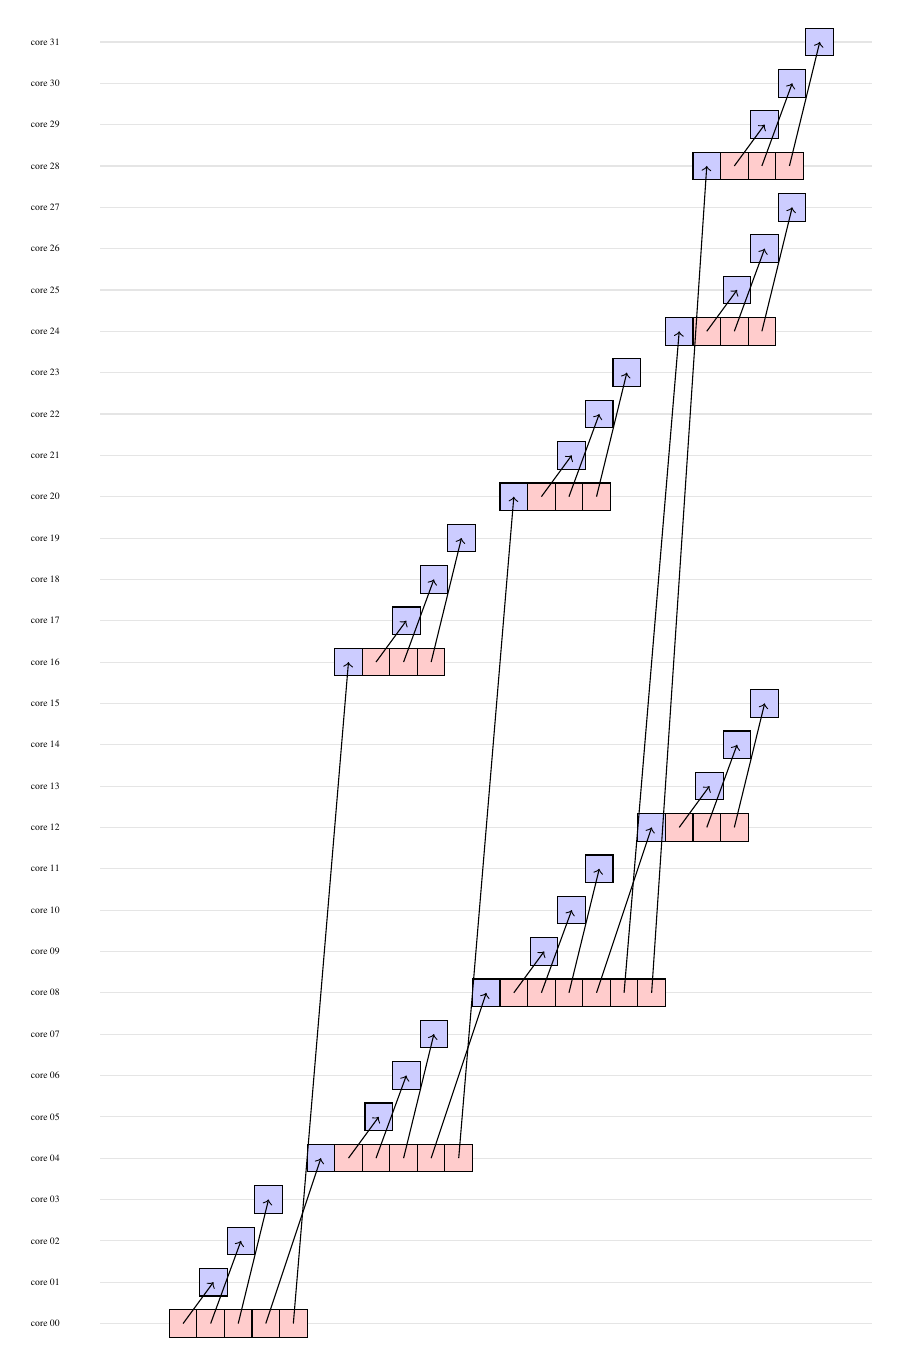
\begin{tikzpicture}[scale=.35,transform shape]
    % Insert visualization
    \node at (0mm,0mm) {core 00};
\draw[color=black!10] (20mm,0mm) -- (30cm,0mm);
\node at (0mm,15mm) {core 01};
\draw[color=black!10] (20mm,15mm) -- (30cm,15mm);
\node at (0mm,30mm) {core 02};
\draw[color=black!10] (20mm,30mm) -- (30cm,30mm);
\node at (0mm,45mm) {core 03};
\draw[color=black!10] (20mm,45mm) -- (30cm,45mm);
\node at (0mm,60mm) {core 04};
\draw[color=black!10] (20mm,60mm) -- (30cm,60mm);
\node at (0mm,75mm) {core 05};
\draw[color=black!10] (20mm,75mm) -- (30cm,75mm);
\node at (0mm,90mm) {core 06};
\draw[color=black!10] (20mm,90mm) -- (30cm,90mm);
\node at (0mm,105mm) {core 07};
\draw[color=black!10] (20mm,105mm) -- (30cm,105mm);
\node at (0mm,120mm) {core 08};
\draw[color=black!10] (20mm,120mm) -- (30cm,120mm);
\node at (0mm,135mm) {core 09};
\draw[color=black!10] (20mm,135mm) -- (30cm,135mm);
\node at (0mm,150mm) {core 10};
\draw[color=black!10] (20mm,150mm) -- (30cm,150mm);
\node at (0mm,165mm) {core 11};
\draw[color=black!10] (20mm,165mm) -- (30cm,165mm);
\node at (0mm,180mm) {core 12};
\draw[color=black!10] (20mm,180mm) -- (30cm,180mm);
\node at (0mm,195mm) {core 13};
\draw[color=black!10] (20mm,195mm) -- (30cm,195mm);
\node at (0mm,210mm) {core 14};
\draw[color=black!10] (20mm,210mm) -- (30cm,210mm);
\node at (0mm,225mm) {core 15};
\draw[color=black!10] (20mm,225mm) -- (30cm,225mm);
\node at (0mm,240mm) {core 16};
\draw[color=black!10] (20mm,240mm) -- (30cm,240mm);
\node at (0mm,255mm) {core 17};
\draw[color=black!10] (20mm,255mm) -- (30cm,255mm);
\node at (0mm,270mm) {core 18};
\draw[color=black!10] (20mm,270mm) -- (30cm,270mm);
\node at (0mm,285mm) {core 19};
\draw[color=black!10] (20mm,285mm) -- (30cm,285mm);
\node at (0mm,300mm) {core 20};
\draw[color=black!10] (20mm,300mm) -- (30cm,300mm);
\node at (0mm,315mm) {core 21};
\draw[color=black!10] (20mm,315mm) -- (30cm,315mm);
\node at (0mm,330mm) {core 22};
\draw[color=black!10] (20mm,330mm) -- (30cm,330mm);
\node at (0mm,345mm) {core 23};
\draw[color=black!10] (20mm,345mm) -- (30cm,345mm);
\node at (0mm,360mm) {core 24};
\draw[color=black!10] (20mm,360mm) -- (30cm,360mm);
\node at (0mm,375mm) {core 25};
\draw[color=black!10] (20mm,375mm) -- (30cm,375mm);
\node at (0mm,390mm) {core 26};
\draw[color=black!10] (20mm,390mm) -- (30cm,390mm);
\node at (0mm,405mm) {core 27};
\draw[color=black!10] (20mm,405mm) -- (30cm,405mm);
\node at (0mm,420mm) {core 28};
\draw[color=black!10] (20mm,420mm) -- (30cm,420mm);
\node at (0mm,435mm) {core 29};
\draw[color=black!10] (20mm,435mm) -- (30cm,435mm);
\node at (0mm,450mm) {core 30};
\draw[color=black!10] (20mm,450mm) -- (30cm,450mm);
\node at (0mm,465mm) {core 31};
\draw[color=black!10] (20mm,465mm) -- (30cm,465mm);
\node[draw,fill=red!20,minimum size=10mm] (s_0_1) at (50mm,0mm) {};
\node[draw,fill=red!20,minimum size=10mm] (s_0_2) at (60mm,0mm) {};
\node[draw,fill=red!20,minimum size=10mm] (s_0_3) at (70mm,0mm) {};
\node[draw,fill=red!20,minimum size=10mm] (s_0_4) at (80mm,0mm) {};
\node[draw,fill=red!20,minimum size=10mm] (s_0_16) at (90mm,0mm) {};
\node[draw,fill=blue!20,minimum size=10mm] (r_0_1) at (61mm,15mm) {};
\draw[->] (s_0_1.center) -- (r_0_1.center); 
\node[draw,fill=blue!20,minimum size=10mm] (r_0_2) at (71mm,30mm) {};
\draw[->] (s_0_2.center) -- (r_0_2.center); 
\node[draw,fill=blue!20,minimum size=10mm] (r_0_3) at (81mm,45mm) {};
\draw[->] (s_0_3.center) -- (r_0_3.center); 
\node[draw,fill=blue!20,minimum size=10mm] (r_0_4) at (100mm,60mm) {};
\draw[->] (s_0_4.center) -- (r_0_4.center); 
\node[draw,fill=red!20,minimum size=10mm] (s_4_5) at (110mm,60mm) {};
\node[draw,fill=red!20,minimum size=10mm] (s_4_6) at (120mm,60mm) {};
\node[draw,fill=red!20,minimum size=10mm] (s_4_7) at (130mm,60mm) {};
\node[draw,fill=red!20,minimum size=10mm] (s_4_8) at (140mm,60mm) {};
\node[draw,fill=red!20,minimum size=10mm] (s_4_20) at (150mm,60mm) {};
\node[draw,fill=blue!20,minimum size=10mm] (r_0_16) at (110mm,240mm) {};
\draw[->] (s_0_16.center) -- (r_0_16.center); 
\node[draw,fill=red!20,minimum size=10mm] (s_16_17) at (120mm,240mm) {};
\node[draw,fill=red!20,minimum size=10mm] (s_16_18) at (130mm,240mm) {};
\node[draw,fill=red!20,minimum size=10mm] (s_16_19) at (140mm,240mm) {};
\node[draw,fill=blue!20,minimum size=10mm] (r_4_5) at (121mm,75mm) {};
\draw[->] (s_4_5.center) -- (r_4_5.center); 
\node[draw,fill=blue!20,minimum size=10mm] (r_16_17) at (131mm,255mm) {};
\draw[->] (s_16_17.center) -- (r_16_17.center); 
\node[draw,fill=blue!20,minimum size=10mm] (r_4_6) at (131mm,90mm) {};
\draw[->] (s_4_6.center) -- (r_4_6.center); 
\node[draw,fill=blue!20,minimum size=10mm] (r_16_18) at (141mm,270mm) {};
\draw[->] (s_16_18.center) -- (r_16_18.center); 
\node[draw,fill=blue!20,minimum size=10mm] (r_4_7) at (141mm,105mm) {};
\draw[->] (s_4_7.center) -- (r_4_7.center); 
\node[draw,fill=blue!20,minimum size=10mm] (r_16_19) at (151mm,285mm) {};
\draw[->] (s_16_19.center) -- (r_16_19.center); 
\node[draw,fill=blue!20,minimum size=10mm] (r_4_8) at (160mm,120mm) {};
\draw[->] (s_4_8.center) -- (r_4_8.center); 
\node[draw,fill=red!20,minimum size=10mm] (s_8_9) at (170mm,120mm) {};
\node[draw,fill=red!20,minimum size=10mm] (s_8_10) at (180mm,120mm) {};
\node[draw,fill=red!20,minimum size=10mm] (s_8_11) at (190mm,120mm) {};
\node[draw,fill=red!20,minimum size=10mm] (s_8_12) at (200mm,120mm) {};
\node[draw,fill=red!20,minimum size=10mm] (s_8_24) at (210mm,120mm) {};
\node[draw,fill=red!20,minimum size=10mm] (s_8_28) at (220mm,120mm) {};
\node[draw,fill=blue!20,minimum size=10mm] (r_4_20) at (170mm,300mm) {};
\draw[->] (s_4_20.center) -- (r_4_20.center); 
\node[draw,fill=red!20,minimum size=10mm] (s_20_21) at (180mm,300mm) {};
\node[draw,fill=red!20,minimum size=10mm] (s_20_22) at (190mm,300mm) {};
\node[draw,fill=red!20,minimum size=10mm] (s_20_23) at (200mm,300mm) {};
\node[draw,fill=blue!20,minimum size=10mm] (r_8_9) at (181mm,135mm) {};
\draw[->] (s_8_9.center) -- (r_8_9.center); 
\node[draw,fill=blue!20,minimum size=10mm] (r_20_21) at (191mm,315mm) {};
\draw[->] (s_20_21.center) -- (r_20_21.center); 
\node[draw,fill=blue!20,minimum size=10mm] (r_8_10) at (191mm,150mm) {};
\draw[->] (s_8_10.center) -- (r_8_10.center); 
\node[draw,fill=blue!20,minimum size=10mm] (r_20_22) at (201mm,330mm) {};
\draw[->] (s_20_22.center) -- (r_20_22.center); 
\node[draw,fill=blue!20,minimum size=10mm] (r_8_11) at (201mm,165mm) {};
\draw[->] (s_8_11.center) -- (r_8_11.center); 
\node[draw,fill=blue!20,minimum size=10mm] (r_20_23) at (211mm,345mm) {};
\draw[->] (s_20_23.center) -- (r_20_23.center); 
\node[draw,fill=blue!20,minimum size=10mm] (r_8_12) at (220mm,180mm) {};
\draw[->] (s_8_12.center) -- (r_8_12.center); 
\node[draw,fill=red!20,minimum size=10mm] (s_12_13) at (230mm,180mm) {};
\node[draw,fill=red!20,minimum size=10mm] (s_12_14) at (240mm,180mm) {};
\node[draw,fill=red!20,minimum size=10mm] (s_12_15) at (250mm,180mm) {};
\node[draw,fill=blue!20,minimum size=10mm] (r_8_24) at (230mm,360mm) {};
\draw[->] (s_8_24.center) -- (r_8_24.center); 
\node[draw,fill=red!20,minimum size=10mm] (s_24_25) at (240mm,360mm) {};
\node[draw,fill=red!20,minimum size=10mm] (s_24_26) at (250mm,360mm) {};
\node[draw,fill=red!20,minimum size=10mm] (s_24_27) at (260mm,360mm) {};
\node[draw,fill=blue!20,minimum size=10mm] (r_8_28) at (240mm,420mm) {};
\draw[->] (s_8_28.center) -- (r_8_28.center); 
\node[draw,fill=red!20,minimum size=10mm] (s_28_29) at (250mm,420mm) {};
\node[draw,fill=red!20,minimum size=10mm] (s_28_30) at (260mm,420mm) {};
\node[draw,fill=red!20,minimum size=10mm] (s_28_31) at (270mm,420mm) {};
\node[draw,fill=blue!20,minimum size=10mm] (r_12_13) at (241mm,195mm) {};
\draw[->] (s_12_13.center) -- (r_12_13.center); 
\node[draw,fill=blue!20,minimum size=10mm] (r_12_14) at (251mm,210mm) {};
\draw[->] (s_12_14.center) -- (r_12_14.center); 
\node[draw,fill=blue!20,minimum size=10mm] (r_24_25) at (251mm,375mm) {};
\draw[->] (s_24_25.center) -- (r_24_25.center); 
\node[draw,fill=blue!20,minimum size=10mm] (r_28_29) at (261mm,435mm) {};
\draw[->] (s_28_29.center) -- (r_28_29.center); 
\node[draw,fill=blue!20,minimum size=10mm] (r_24_26) at (261mm,390mm) {};
\draw[->] (s_24_26.center) -- (r_24_26.center); 
\node[draw,fill=blue!20,minimum size=10mm] (r_12_15) at (261mm,225mm) {};
\draw[->] (s_12_15.center) -- (r_12_15.center); 
\node[draw,fill=blue!20,minimum size=10mm] (r_28_30) at (271mm,450mm) {};
\draw[->] (s_28_30.center) -- (r_28_30.center); 
\node[draw,fill=blue!20,minimum size=10mm] (r_24_27) at (271mm,405mm) {};
\draw[->] (s_24_27.center) -- (r_24_27.center); 
\node[draw,fill=blue!20,minimum size=10mm] (r_28_31) at (281mm,465mm) {};
\draw[->] (s_28_31.center) -- (r_28_31.center); 

  \end{tikzpicture}
  \caption{Visualization of operations for sending a message along the
    tree. Red boxes represent send operations, blue boxes represent
    receive operations and arrows messages sent between cores. The
    tree has been acquired using an MST algorithm.}
  \label{fig:mst_gruyere_operations}
\end{figure}

In Figure~\ref{fig:mst_gruyere_operations_sorted} we schedule sending
of messages based on link cost. We sort the outgoing edges by their
weights and send on the most expensive links first. See
Algorithm~\ref{algo:scheduling_link_weight}

\begin{algorithm}[htb]
\SetCommentSty{textc}
\SetKwFunction{weight}{edge\_weight}%
\SetKwFunction{sort}{sort\_by\_edge\_weight}%
\SetKwFunction{icsend}{send}%
  %
  \KwData{Node $n$ sending messages, \\ %
    broadcast tree as graph $(V, E)$, \\ %
    weight function \weight{$E$}
    %
  }
  % 
  \BlankLine
  $nb \leftarrow \{ c: \exists (self, c) \in E \}$\tcp*{Get children}
  $nb \leftarrow $ \sort{$nb$, \weight{}}\tcp*{Sort by edge weight}
  \For(\tcp*{For all children}){$c \leftarrow nb$}{
    \icsend{$c$}
  }
  % 
  \caption{Scheduling in order of outgoing link weight}
  \label{algo:scheduling_link_weight}
\end{algorithm}

\begin{figure}[htb]
  \centering
  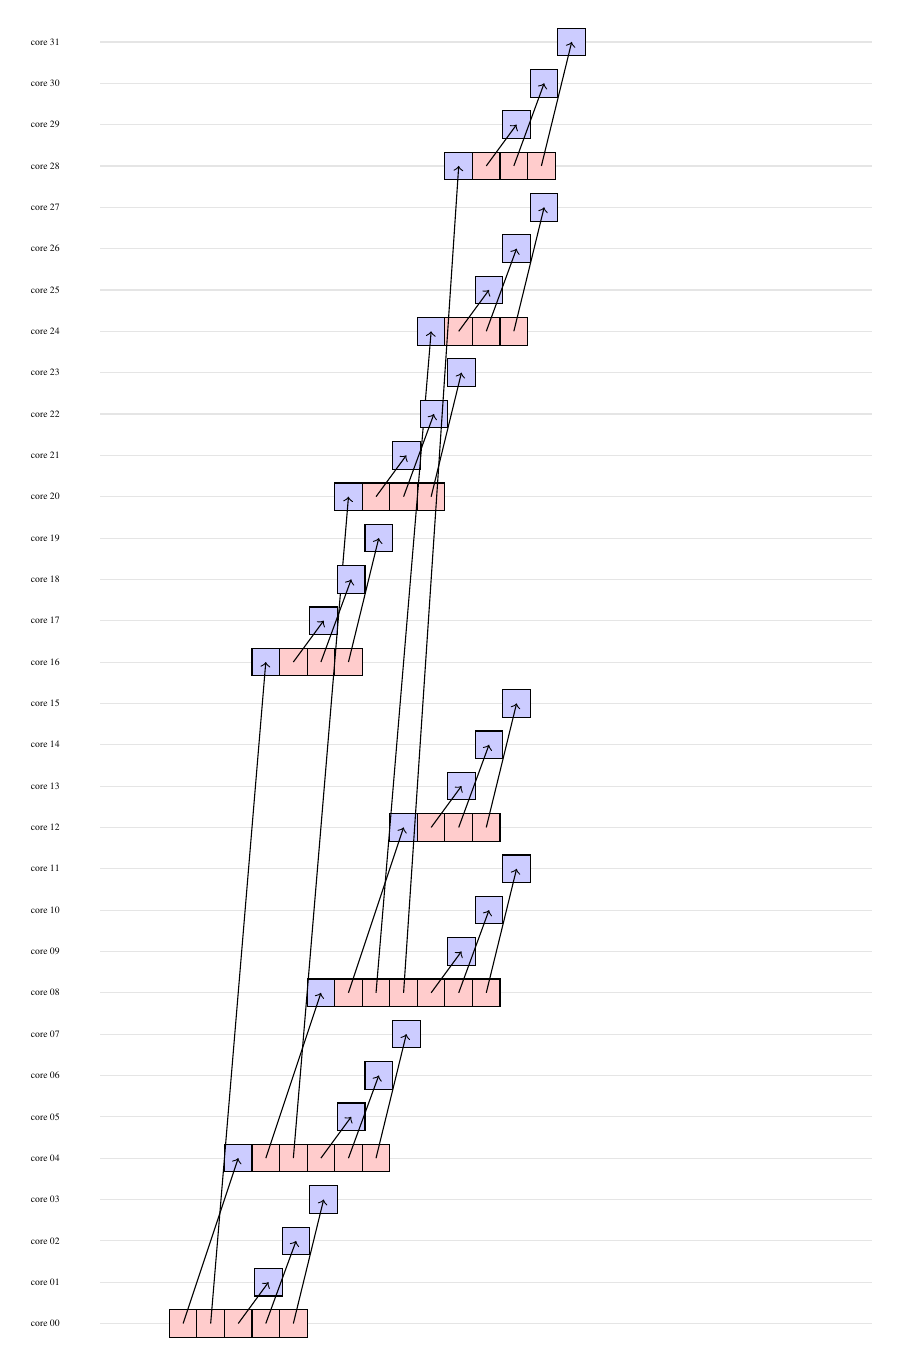
\begin{tikzpicture}[scale=.35,transform shape]
    % Insert visualization
    \node at (0mm,0mm) {core 00};
\draw[color=black!10] (20mm,0mm) -- (30cm,0mm);
\node at (0mm,15mm) {core 01};
\draw[color=black!10] (20mm,15mm) -- (30cm,15mm);
\node at (0mm,30mm) {core 02};
\draw[color=black!10] (20mm,30mm) -- (30cm,30mm);
\node at (0mm,45mm) {core 03};
\draw[color=black!10] (20mm,45mm) -- (30cm,45mm);
\node at (0mm,60mm) {core 04};
\draw[color=black!10] (20mm,60mm) -- (30cm,60mm);
\node at (0mm,75mm) {core 05};
\draw[color=black!10] (20mm,75mm) -- (30cm,75mm);
\node at (0mm,90mm) {core 06};
\draw[color=black!10] (20mm,90mm) -- (30cm,90mm);
\node at (0mm,105mm) {core 07};
\draw[color=black!10] (20mm,105mm) -- (30cm,105mm);
\node at (0mm,120mm) {core 08};
\draw[color=black!10] (20mm,120mm) -- (30cm,120mm);
\node at (0mm,135mm) {core 09};
\draw[color=black!10] (20mm,135mm) -- (30cm,135mm);
\node at (0mm,150mm) {core 10};
\draw[color=black!10] (20mm,150mm) -- (30cm,150mm);
\node at (0mm,165mm) {core 11};
\draw[color=black!10] (20mm,165mm) -- (30cm,165mm);
\node at (0mm,180mm) {core 12};
\draw[color=black!10] (20mm,180mm) -- (30cm,180mm);
\node at (0mm,195mm) {core 13};
\draw[color=black!10] (20mm,195mm) -- (30cm,195mm);
\node at (0mm,210mm) {core 14};
\draw[color=black!10] (20mm,210mm) -- (30cm,210mm);
\node at (0mm,225mm) {core 15};
\draw[color=black!10] (20mm,225mm) -- (30cm,225mm);
\node at (0mm,240mm) {core 16};
\draw[color=black!10] (20mm,240mm) -- (30cm,240mm);
\node at (0mm,255mm) {core 17};
\draw[color=black!10] (20mm,255mm) -- (30cm,255mm);
\node at (0mm,270mm) {core 18};
\draw[color=black!10] (20mm,270mm) -- (30cm,270mm);
\node at (0mm,285mm) {core 19};
\draw[color=black!10] (20mm,285mm) -- (30cm,285mm);
\node at (0mm,300mm) {core 20};
\draw[color=black!10] (20mm,300mm) -- (30cm,300mm);
\node at (0mm,315mm) {core 21};
\draw[color=black!10] (20mm,315mm) -- (30cm,315mm);
\node at (0mm,330mm) {core 22};
\draw[color=black!10] (20mm,330mm) -- (30cm,330mm);
\node at (0mm,345mm) {core 23};
\draw[color=black!10] (20mm,345mm) -- (30cm,345mm);
\node at (0mm,360mm) {core 24};
\draw[color=black!10] (20mm,360mm) -- (30cm,360mm);
\node at (0mm,375mm) {core 25};
\draw[color=black!10] (20mm,375mm) -- (30cm,375mm);
\node at (0mm,390mm) {core 26};
\draw[color=black!10] (20mm,390mm) -- (30cm,390mm);
\node at (0mm,405mm) {core 27};
\draw[color=black!10] (20mm,405mm) -- (30cm,405mm);
\node at (0mm,420mm) {core 28};
\draw[color=black!10] (20mm,420mm) -- (30cm,420mm);
\node at (0mm,435mm) {core 29};
\draw[color=black!10] (20mm,435mm) -- (30cm,435mm);
\node at (0mm,450mm) {core 30};
\draw[color=black!10] (20mm,450mm) -- (30cm,450mm);
\node at (0mm,465mm) {core 31};
\draw[color=black!10] (20mm,465mm) -- (30cm,465mm);
\node[draw,fill=red!20,minimum size=10mm] (s_0_4) at (50mm,0mm) {};
\node[draw,fill=red!20,minimum size=10mm] (s_0_16) at (60mm,0mm) {};
\node[draw,fill=red!20,minimum size=10mm] (s_0_1) at (70mm,0mm) {};
\node[draw,fill=red!20,minimum size=10mm] (s_0_2) at (80mm,0mm) {};
\node[draw,fill=red!20,minimum size=10mm] (s_0_3) at (90mm,0mm) {};
\node[draw,fill=blue!20,minimum size=10mm] (r_0_4) at (70mm,60mm) {};
\draw[->] (s_0_4.center) -- (r_0_4.center); 
\node[draw,fill=red!20,minimum size=10mm] (s_4_8) at (80mm,60mm) {};
\node[draw,fill=red!20,minimum size=10mm] (s_4_20) at (90mm,60mm) {};
\node[draw,fill=red!20,minimum size=10mm] (s_4_5) at (100mm,60mm) {};
\node[draw,fill=red!20,minimum size=10mm] (s_4_6) at (110mm,60mm) {};
\node[draw,fill=red!20,minimum size=10mm] (s_4_7) at (120mm,60mm) {};
\node[draw,fill=blue!20,minimum size=10mm] (r_0_16) at (80mm,240mm) {};
\draw[->] (s_0_16.center) -- (r_0_16.center); 
\node[draw,fill=red!20,minimum size=10mm] (s_16_17) at (90mm,240mm) {};
\node[draw,fill=red!20,minimum size=10mm] (s_16_18) at (100mm,240mm) {};
\node[draw,fill=red!20,minimum size=10mm] (s_16_19) at (110mm,240mm) {};
\node[draw,fill=blue!20,minimum size=10mm] (r_0_1) at (81mm,15mm) {};
\draw[->] (s_0_1.center) -- (r_0_1.center); 
\node[draw,fill=blue!20,minimum size=10mm] (r_0_2) at (91mm,30mm) {};
\draw[->] (s_0_2.center) -- (r_0_2.center); 
\node[draw,fill=blue!20,minimum size=10mm] (r_4_8) at (100mm,120mm) {};
\draw[->] (s_4_8.center) -- (r_4_8.center); 
\node[draw,fill=red!20,minimum size=10mm] (s_8_12) at (110mm,120mm) {};
\node[draw,fill=red!20,minimum size=10mm] (s_8_24) at (120mm,120mm) {};
\node[draw,fill=red!20,minimum size=10mm] (s_8_28) at (130mm,120mm) {};
\node[draw,fill=red!20,minimum size=10mm] (s_8_9) at (140mm,120mm) {};
\node[draw,fill=red!20,minimum size=10mm] (s_8_10) at (150mm,120mm) {};
\node[draw,fill=red!20,minimum size=10mm] (s_8_11) at (160mm,120mm) {};
\node[draw,fill=blue!20,minimum size=10mm] (r_0_3) at (101mm,45mm) {};
\draw[->] (s_0_3.center) -- (r_0_3.center); 
\node[draw,fill=blue!20,minimum size=10mm] (r_16_17) at (101mm,255mm) {};
\draw[->] (s_16_17.center) -- (r_16_17.center); 
\node[draw,fill=blue!20,minimum size=10mm] (r_4_20) at (110mm,300mm) {};
\draw[->] (s_4_20.center) -- (r_4_20.center); 
\node[draw,fill=red!20,minimum size=10mm] (s_20_21) at (120mm,300mm) {};
\node[draw,fill=red!20,minimum size=10mm] (s_20_22) at (130mm,300mm) {};
\node[draw,fill=red!20,minimum size=10mm] (s_20_23) at (140mm,300mm) {};
\node[draw,fill=blue!20,minimum size=10mm] (r_4_5) at (111mm,75mm) {};
\draw[->] (s_4_5.center) -- (r_4_5.center); 
\node[draw,fill=blue!20,minimum size=10mm] (r_16_18) at (111mm,270mm) {};
\draw[->] (s_16_18.center) -- (r_16_18.center); 
\node[draw,fill=blue!20,minimum size=10mm] (r_4_6) at (121mm,90mm) {};
\draw[->] (s_4_6.center) -- (r_4_6.center); 
\node[draw,fill=blue!20,minimum size=10mm] (r_16_19) at (121mm,285mm) {};
\draw[->] (s_16_19.center) -- (r_16_19.center); 
\node[draw,fill=blue!20,minimum size=10mm] (r_8_12) at (130mm,180mm) {};
\draw[->] (s_8_12.center) -- (r_8_12.center); 
\node[draw,fill=red!20,minimum size=10mm] (s_12_13) at (140mm,180mm) {};
\node[draw,fill=red!20,minimum size=10mm] (s_12_14) at (150mm,180mm) {};
\node[draw,fill=red!20,minimum size=10mm] (s_12_15) at (160mm,180mm) {};
\node[draw,fill=blue!20,minimum size=10mm] (r_20_21) at (131mm,315mm) {};
\draw[->] (s_20_21.center) -- (r_20_21.center); 
\node[draw,fill=blue!20,minimum size=10mm] (r_4_7) at (131mm,105mm) {};
\draw[->] (s_4_7.center) -- (r_4_7.center); 
\node[draw,fill=blue!20,minimum size=10mm] (r_8_24) at (140mm,360mm) {};
\draw[->] (s_8_24.center) -- (r_8_24.center); 
\node[draw,fill=red!20,minimum size=10mm] (s_24_25) at (150mm,360mm) {};
\node[draw,fill=red!20,minimum size=10mm] (s_24_26) at (160mm,360mm) {};
\node[draw,fill=red!20,minimum size=10mm] (s_24_27) at (170mm,360mm) {};
\node[draw,fill=blue!20,minimum size=10mm] (r_20_22) at (141mm,330mm) {};
\draw[->] (s_20_22.center) -- (r_20_22.center); 
\node[draw,fill=blue!20,minimum size=10mm] (r_8_28) at (150mm,420mm) {};
\draw[->] (s_8_28.center) -- (r_8_28.center); 
\node[draw,fill=red!20,minimum size=10mm] (s_28_29) at (160mm,420mm) {};
\node[draw,fill=red!20,minimum size=10mm] (s_28_30) at (170mm,420mm) {};
\node[draw,fill=red!20,minimum size=10mm] (s_28_31) at (180mm,420mm) {};
\node[draw,fill=blue!20,minimum size=10mm] (r_20_23) at (151mm,345mm) {};
\draw[->] (s_20_23.center) -- (r_20_23.center); 
\node[draw,fill=blue!20,minimum size=10mm] (r_12_13) at (151mm,195mm) {};
\draw[->] (s_12_13.center) -- (r_12_13.center); 
\node[draw,fill=blue!20,minimum size=10mm] (r_8_9) at (151mm,135mm) {};
\draw[->] (s_8_9.center) -- (r_8_9.center); 
\node[draw,fill=blue!20,minimum size=10mm] (r_12_14) at (161mm,210mm) {};
\draw[->] (s_12_14.center) -- (r_12_14.center); 
\node[draw,fill=blue!20,minimum size=10mm] (r_8_10) at (161mm,150mm) {};
\draw[->] (s_8_10.center) -- (r_8_10.center); 
\node[draw,fill=blue!20,minimum size=10mm] (r_24_25) at (161mm,375mm) {};
\draw[->] (s_24_25.center) -- (r_24_25.center); 
\node[draw,fill=blue!20,minimum size=10mm] (r_28_29) at (171mm,435mm) {};
\draw[->] (s_28_29.center) -- (r_28_29.center); 
\node[draw,fill=blue!20,minimum size=10mm] (r_12_15) at (171mm,225mm) {};
\draw[->] (s_12_15.center) -- (r_12_15.center); 
\node[draw,fill=blue!20,minimum size=10mm] (r_24_26) at (171mm,390mm) {};
\draw[->] (s_24_26.center) -- (r_24_26.center); 
\node[draw,fill=blue!20,minimum size=10mm] (r_8_11) at (171mm,165mm) {};
\draw[->] (s_8_11.center) -- (r_8_11.center); 
\node[draw,fill=blue!20,minimum size=10mm] (r_28_30) at (181mm,450mm) {};
\draw[->] (s_28_30.center) -- (r_28_30.center); 
\node[draw,fill=blue!20,minimum size=10mm] (r_24_27) at (181mm,405mm) {};
\draw[->] (s_24_27.center) -- (r_24_27.center); 
\node[draw,fill=blue!20,minimum size=10mm] (r_28_31) at (191mm,465mm) {};
\draw[->] (s_28_31.center) -- (r_28_31.center); 

  \end{tikzpicture}
  \caption{Visualization of operations for sending a message along the
    tree. Red boxes represent send operations, blue boxes represent
    receive operations and arrows messages sent between cores. After
    running the MST algorithm, we optimize scheduling in every node to
    send messages to in decreasing order of their latency.}
  \label{fig:mst_gruyere_operations_sorted}
\end{figure}

%%%%%%%%%%%%%%%%%%%%%%%%%%%%%%%%%%%%%%%%%%%%%%%%%%
\section{Implementation}

% Our implementation
Assuming the tree, we now implement an atomic broadcast for multicore
machines. Our implementation is based on the Barrelfish UMP
interconnect driver. It provides reliable channels with in-order
delivery. Flow control is build in for reliability. Communication
starts at the root node, which acts as a
sequentializer. See~\ref{algo:ab} for details.

\begin{algorithm}[htb]
\SetCommentSty{textc}
\SetKwInOut{Assumptions}{assumptions}
\Assumptions{Underlying communication channel is reliable and in-order}
\SetKwProg{Fn}{Function}{}{end}%
\SetKwFunction{receive}{on\_receive}%
\SetKwFunction{waitchild}{wait\_for\_children}%
\SetKwFunction{send}{send}%
\SetKwFunction{icsend}{send\_bc\_request}%
\SetKwFunction{icsendack}{send\_bc\_ack}%
\SetKwFunction{handlemessages}{handle\_other\_messages}%
  %
  \KwData{List of processes $p$, broadcast tree as graph $(V, E)$}
  \KwResult{Tree based atomic broadcast using a sequentializer}
  % 
  \BlankLine
  \Fn(\tcp*{Receive a message}){\receive{$client$, $m$}}{
    \For(\tcp*{For all children}){$c \leftarrow \{ c: \exists (self, c) \in E \} $}{
      \icsend{c}
    }
    \waitchild{}\;
    \icsendack{$client$}\;
  }
  % 
  \BlankLine
  \Fn(\tcp*{Send a message}){\send{void}}{
    \tcc{Need to wait for acknowledgment before returning to
      caller. Otherwise, sender might see his own request before some
      other request, that the sequentializer decided to handle first}
    \icsend{$V_{root}$}\tcp*{Relay msg (sequentializer)}
    \While{no answer received}{
      \handlemessages{}\tcp*{Otherwise, deadlocks}
    }
  }
  \caption{Atomic broadcast on reliable communication channels}
  \label{algo:ab}

\end{algorithm}

%%%%%%%%%%%%%%%%%%%%%%%%%%%%%%%%%%%%%%%%%%%%%%%%%%
\subsection{Issues with the Barrelfish implementation}

When implementing the protocol in Barrelfish, we found several
practical problems, which we will discuss briefly in this section.
We kick-start our protocol connecting every process with all other
processes to get a fully-meshed network of channels.
We use a round-based algorithm to open channels. Then, every node
knows exactly the source of an incoming connection. We formalize this
algorithm in Algorithm~\ref{algo:ab_bind}.
This is required for Barrelfish UMP communication channels since on
bind, no source identifier is send along\footnote{Check if this is
  actually true, and even if it is true, if is a Barrelfish problem,
  and not a general one}.

\begin{algorithm}[htb]
  %
  \SetKwInOut{Assumptions}{assumptions}
  \Assumptions{Processes have unique contiguous
    identifiers starting at 0}
  \BlankLine
  %
  \SetKwArray{c}{channels}
  \SetKwFunction{connectNode}{connectNode}
  \SetKwFunction{listen}{listen}
  \SetKwFunction{barrier}{barrier}
  % 
  \KwData{process id $p$, round $r$, %
    each process an array of channels \c}
  \KwResult{Fully-meshed network of processes}
  % 
  \BlankLine
  %
  $r \leftarrow 0$\;
  \For{$i \leftarrow 0$ \KwTo $num(p)$}{
    \eIf{$p=i$}{
      \For{$o \leftarrow i+1$ \KwTo $num(p)$}{
        \c{$o$} $\leftarrow$ \connectNode{$o$}\;
      }
    }{
        \c{$i$} $\leftarrow$ \listen{}\;
    }
    \barrier{} \tcp*{Otherwise, reordering possible}
  }
  \caption{Establish fully-meshed network of channels}
  \label{algo:ab_bind}
\end{algorithm}

%%%%%%%%%%%%%%%%%%%%%%%%%%%%%%%%%%%%%%%%%%%%%%%%%%
%%%%%%%%%%%%%%%%%%%%%%%%%%%%%%%%%%%%%%%%%%%%%%%%%%
\section{Evaluation}

\stefan{Compare to pure shared-memory implementations, otherwise
  reviewers might argue that there is no need for distributed
  algorithms.}

%%%%%%%%%%%%%%%%%%%%%%%%%%%%%%%%%%%%%%%%%%%%%%%%%%
\subsection{Atomic broadcast}

%-------------------------------------------------
\subsubsection{Simulation}

This section shows results for a simulation based on the model
introduced in Section~\ref{sec:mst_tree}. The time given is a
fictional time unit at this point.

\begin{table}[htb]
  \centering
  \begin{tabular}{llll}
    \toprule
    topology & scheduling & time & factor \\
    \midrule
    MST & naive         & 241 & 1.00 \\
    MST & longest first & 151 & 0.63 \\
    \bottomrule
  \end{tabular}
  \caption{Simulation results for simplified machine model}
  \label{tab:sim_results}
\end{table}

%-------------------------------------------------
\subsubsection{Real hardware}

Current numbers are listed in Table~\ref{tab:bc_measurements}.

\begin{table}[htb]
  \centering
  \begin{tabular}{lrrrr}
    \toprule
    broadcast algorithm & \multicolumn{2}{c}{nos5} & \multicolumn{2}{c}{gruyere} \\
      & cycles & error & cycles & error \\
    \midrule
    sequential &  4096.1 &  105.2 & 136751.9 &   3061.5 \\
    batch      &  2408.0 &  181.9 &  57360.8 &   5271.5 \\
    \bottomrule
  \end{tabular}
  \caption{Broadcast measurements}
  \label{tab:bc_measurements}
\end{table}

Plot~\ref{pgfplot:201303141819} shows the cost of flooding a sub-tree
(with the 50\% worst measurements dropped). The group communication is
based on a binary tree. Core 0 is the root, cores 1 and 2 are its
children etc.

The average cost is really high (probably a scheduling issue). But the
minimal numbers show what is possible. The numbers achieved are easily
explainable. The cost is increasing logarithmic with the number of
nodes reached by the broadcast (as expected). Every level in the tree
adds an additional 2500 to 3000 cycles to the tree. Node 0 takes
significantly longer. I don't know yet why that is.

\begin{figure}
  \caption{Execution time for a broadcast with ACK on gruyere. The
    cost is for execution for the sub-graph starting at the given
    node. Refer to Figure~\ref{fig:qrm_tree_gruyere} for a
    visualization of the broadcast tree used. }
  \label{pgfplot:201303141819}
  \begin{tikzpicture}
    \begin{axis}[
      xlabel=core id,
      scaled y ticks = false, % prevent 10^x stuff
      y tick label style={/pgf/number format/fixed},
      ylabel={cost for subtree [cycles]}]
    \addplot[
      color=red,
      very thin,
      mark=*,
      mark options={%
        scale=.4
      },
      error bars/y dir=both,
      error bars/y explicit] coordinates {
      (0,9932.3) +- (564.4,564.4)
      (1,8240.1) +- (298.5,298.5)
      (2,8259.6) +- (549.4,549.4)
      (3,6206.3) +- (225.1,225.1)
      (4,5914.9) +- (399.2,399.2)
      (5,6033.5) +- (462.2,462.2)
      (6,6070.4) +- (434.3,434.3)
      (7,4530.4) +- (188.6,188.6)
      (8,3163.4) +- (246.1,246.1)
      (9,3403.0) +- (285.3,285.3)
      (10,3650.7) +- (336.5,336.5)
      (11,3559.0) +- (318.8,318.8)
      (12,3558.1) +- (284.8,284.8)
      (13,3567.5) +- (304.5,304.5)
      (14,3476.3) +- (290.2,290.2)
      (15,2711.7) +- (151.9,151.9)
      (16,614.0) +- (17.5,17.5)
      (17,606.2) +- (17.3,17.3)
      (18,636.2) +- (72.5,72.5)
      (19,641.3) +- (46.3,46.3)
      (20,583.8) +- (46.7,46.7)
      (21,577.8) +- (38.3,38.3)
      (22,561.8) +- (18.1,18.1)
      (23,603.5) +- (56.6,56.6)
      (24,589.0) +- (33.4,33.4)
      (25,582.9) +- (33.2,33.2)
      (26,571.7) +- (16.3,16.3)
      (27,581.6) +- (36.6,36.6)
      (28,564.0) +- (16.4,16.4)
      (29,564.0) +- (20.8,20.8)
      (30,551.6) +- (13.0,13.0)
      (31,596.2) +- (51.4,51.4)
    };
    \end{axis}
  \end{tikzpicture}

\end{figure}

%%%%%%%%%%%%%%%%%%%%%%%%%%%%%%%%%%%%%%%%%%%%%%%%%%
%%%%%%%%%%%%%%%%%%%%%%%%%%%%%%%%%%%%%%%%%%%%%%%%%%
\section{Future work}

\begin{itemize}
\item Arguing that group communication/atomic broadcast is important
  and showing that we can do it well might be enough (appeal to atomic
  broadcasts as the foundation for other distributed algorithms, and
  the MPI primitives, that can/need to be mapped to
  group-communication (have a list of them)
\item Need higher-level applications, such as:
  \begin{itemize}
  \item capability system? \stefan{Ask Simon how expensive revocation
      currently is}
  \item a database with replication and consistency maintenance
    \begin{itemize}
    \item SharedDB? (buffers between operators, but no synchronization
      except for access to buffers, which are multiple writers, one
      reader)
    \item Crescando (some kind of state machine replication)
    \end{itemize}
  \end{itemize}
\item MPI collectives (as in~\cite{Tu2008})
\item Try other topologies (Frans Kaashoek), e.g.\ rings
\item \emph{Load balancing in a tree} We could build several rings,
  that do not always include all coordinators and work with read- and
  write-sets. We can select these rings such that they nicely
  integrate with the physical topology. They can also have different
  sizes (e.g.\ a smaller one for read operations and larger ones for
  writes).
\item \emph{Aggregation for convergecast} %
  Convergecast is a way of collecting information from nodes (i.e.\ it
  is kind of the reverse of a broadcast). On the return path,
  information can be aggregated. One example is batching, where several
  pieces of information are grouped in the same message to reduce packet
  processing overhead. Another example is aggregation, i.e.\
  pre-processing of data. One example is pre-calculating the average
  value of child messages if the sink node is not interested in
  individual values. %
  Similarly to what has been done in wireless sensor networks (where it
  also matters to reduce the number of messages, but for other reasons:
  power consumption), we can do aggregation in nodes. In difference to
  traditional distributed systems, this works, because it is easy to
  deploy custom software on every node in the network. Classical
  distributed systems do not typically allow this. Furthermore, reducing
  the number of messages at the price of higher complexity does not make
  sense in classical systems. %
  Examples for aggregation: number of nodes agreeing to something, find
  capabilities (concatenate core ids). 
\end{itemize}

%%%%%%%%%%%%%%%%%%%%%%%%%%%%%%%%%%%%%%%%%%%%%%%%%%
\subsection{Octopus}

Octopus is a coordination service implementation for the Barrelfish
Multikernel operating system based on a key-value store
data-backend. It is, however, centralized. The idea is to make Octopus
a decentralized application.

For that, we extend Octopus such that it can be replicated within a
multicore machine. This will retain scalability for future manycore
machines and potentially outperform a centralized version of Octopus
especially in contented systems.

%--------------------------------------------------
\subsubsection{Key-value store}

One foundation block of Octopus is a key-value store. Since there is
only one copy, the data in there is always consistent. If replicated,
some sort of consistency guarantee would have to be implemented. One
example is \emph{linearizability}, i.e.\ ``accesses occur one at a time
in, some sequential order that is consistent with the order of
invocations and responses''~\cite{lynch}.

One concrete idea is to have one copy of the Octopus data-store
replicated on every NUMA node. One core on every node acts as
\emph{coordinator}, we call the other nodes \emph{slaves}.
Coordinators communicate on a ring. Communication on a local NUMA node
can be realized using read-only shared memory for read access. Write
access needs to be globally ordered and hence communication with other
replicas is required. 

Slaves direct their updates to the local coordinator. Coordinators
send the update request $r$ along the ring and wait for them to be
send back. While passing on requests, coordinators can set a flag to
indicate conflicts. A conflict is another colliding request $r_o$ that
is already in flight. I think we will have to send activity vectors
along with this information! Otherwise, the coordinators requesting
$r$ and $r_o$ will both prevent the other thing from happening and
none of them will be applied! Maybe we need a two-phase commit.

The idea of having a ring is somewhat related to SharedDB. It
optimizes for throughput, not latency!

%-------------------------------------------------
\subsubsection{Synchronization}

It is doubtful that a key-value store as a backend for synchronization
primitives makes sense. As we want to show efficiency, we probably
rather want to implement new synchronization algorithms from scratch.

%%%%%%%%%%%%%%%%%%%%%%%%%%%%%%%%%%%%%%%%%%%%%%%%%%
\subsection{Barriers}

The idea is to explore barrier implementations. The idea is to
leverage information about the NUMA topology for better performance of
barrier intensive workloads. Every NUMA node has a coordinator node,
that knows how many threads on that node want to enter the
barrier. There is only local communication (possibly using a
share-memory implementation to exploit the shared cache) until the
point where all NUMA local threads did enter the barrier.  Then there
is ``global'' communication with other coordinators on other nodes
using a message-passing based algorithm. We believe that this scales
better than pure shared-memory implementations due to less
interconnect contention.

We will have to compare the performance of such an implementation with
a purely shared-memory based implementation like pthreads and
something entirely message-passing based like MPI versions.

%%%%%%%%%%%%%%%%%%%%%%%%%%%%%%%%%%%%%%%%%%%%%%%%%%
\newpage
\bibliographystyle{plain}
\bibliography{defs,db,mendeley}

\label{LastPage}

\end{document}
